\subsection{Raspberry Pi Integration}

\begin{figure}[H]
    \centerline{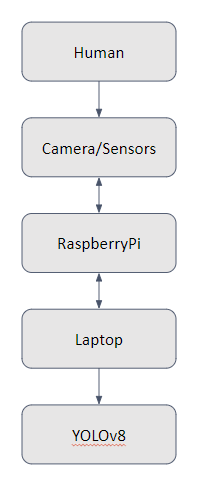
\includegraphics[width=0.1\textwidth]{Figures/Results/Object Detection.png}}
    \caption{Object Detection Flow Chart.}
    \label{fig3a1}
\end{figure}

Fig. ~\ref{fig3a1} shows the flowchart of our object detection with the Raspberry Pi embedded system. As you can see the sequence in the flowchart is by streaming video to Laptop via Raspberry Pi and use YOLOv8 to detect Human.

\begin{figure}[H]
    \centerline{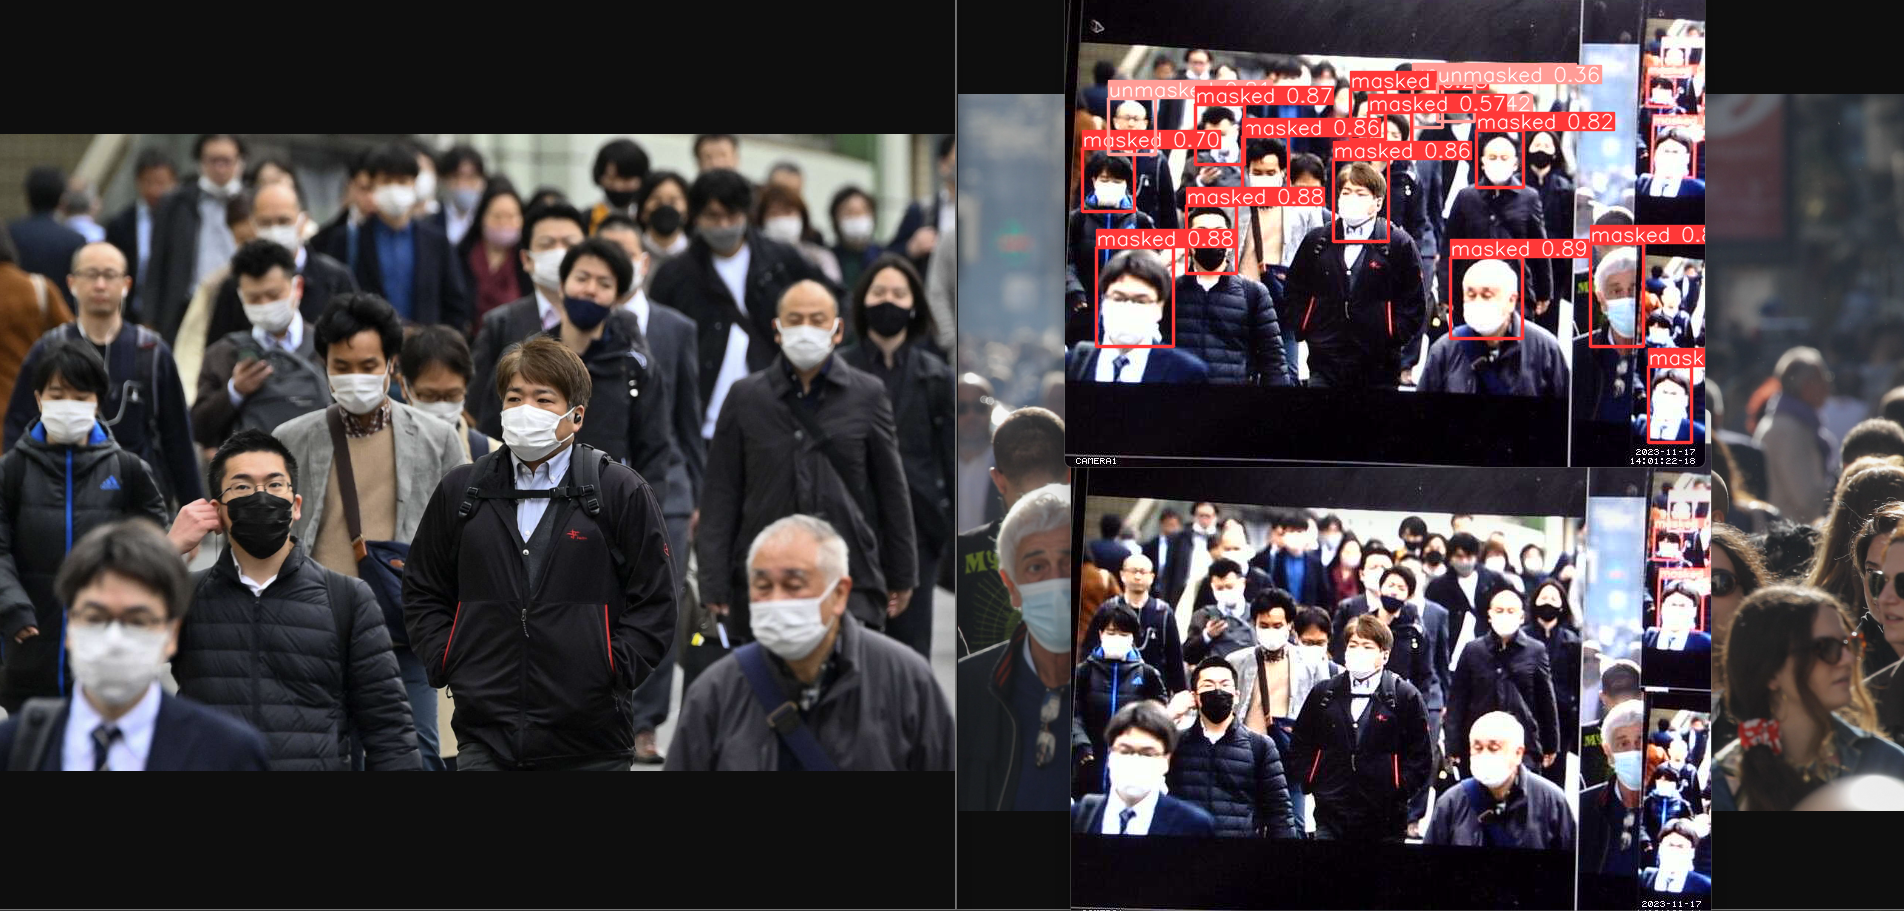
\includegraphics[width=0.5\textwidth]{Figures/Results/RPi_YOLOv8.png}}
    \caption{YOLOv8 model test on real-world dataset with Raspberry Pi 3B.}
    \label{fig3a2}
\end{figure}

Fig. ~\ref{fig3a2} shows the results of real-world dataset testing on the Raspberry Pi 4B using the YOLOv8 model. It can be found that the accuracy is considerable.

As we  we can clearly see the performance differences among them, 
As shown in TABLE \ref{tab1} was the performance difference we had with running Yolov5 on Raspberry Pi 3B, Raspberry Pi 4B. We kept this table here as a referenece and record.
\begin{table}[H]
    \caption{Performance Comparison on running Yolov5}
    \begin{center}
        \resizebox{0.35\textwidth}{!}{%
            \begin{tabular}{|c|c|c|c|}
                \hline
                \textbf{}&\multicolumn{2}{|c|}{\textbf{Controller}} \\
                \cline{2-3} 
                \textbf{Rubric} & \textbf{\textit{RPi3}}& \textbf{\textit{RPi4}} \\
                
                \hline
                CPU (GHz) & 1.2 & 1.5  \\
                \hline
                RAM (GB) & 1 & 8  \\
                \hline
                RAM Usage (MB) & 340 & 332  \\
                \hline
                yolov5s.pt (fps) & 0.21 & 0.95  \\
                \hline
                yolov5n.pt (fps) & 0.43 & 1.67  \\
                \hline
                Load Speed & Very & Very  \\
                (from cmd to start detect) & slow & fast  \\
                
                \hline
            \end{tabular}
        }
        \label{tab1}
    \end{center}
\end{table}

We are also able to control the drone to take off, hover, move in direction, rotation, and landing through Raspberry Pi.